\section{Untersuchung der Kinematik}
Der erste Schritt besteht darin die kinematischen Zusammenhänge des Systems zu analysieren. Im Fall, dass der Würfel auf einer Kante balanciert, verfügt dieser über zwei rotatorische Freiheitsgrade. Der erste wird von der generalisierten Koordinate $\varphi$ beschrieben und gibt die Orientierung des Würfelgehäuses wieder. Die zweite generalisierte Koordinate $\psi$ erfasst die Rotation der Schwungmasse relativ zu dem Würfelgehäuse.
\begin{figure}[!ht]
\centering
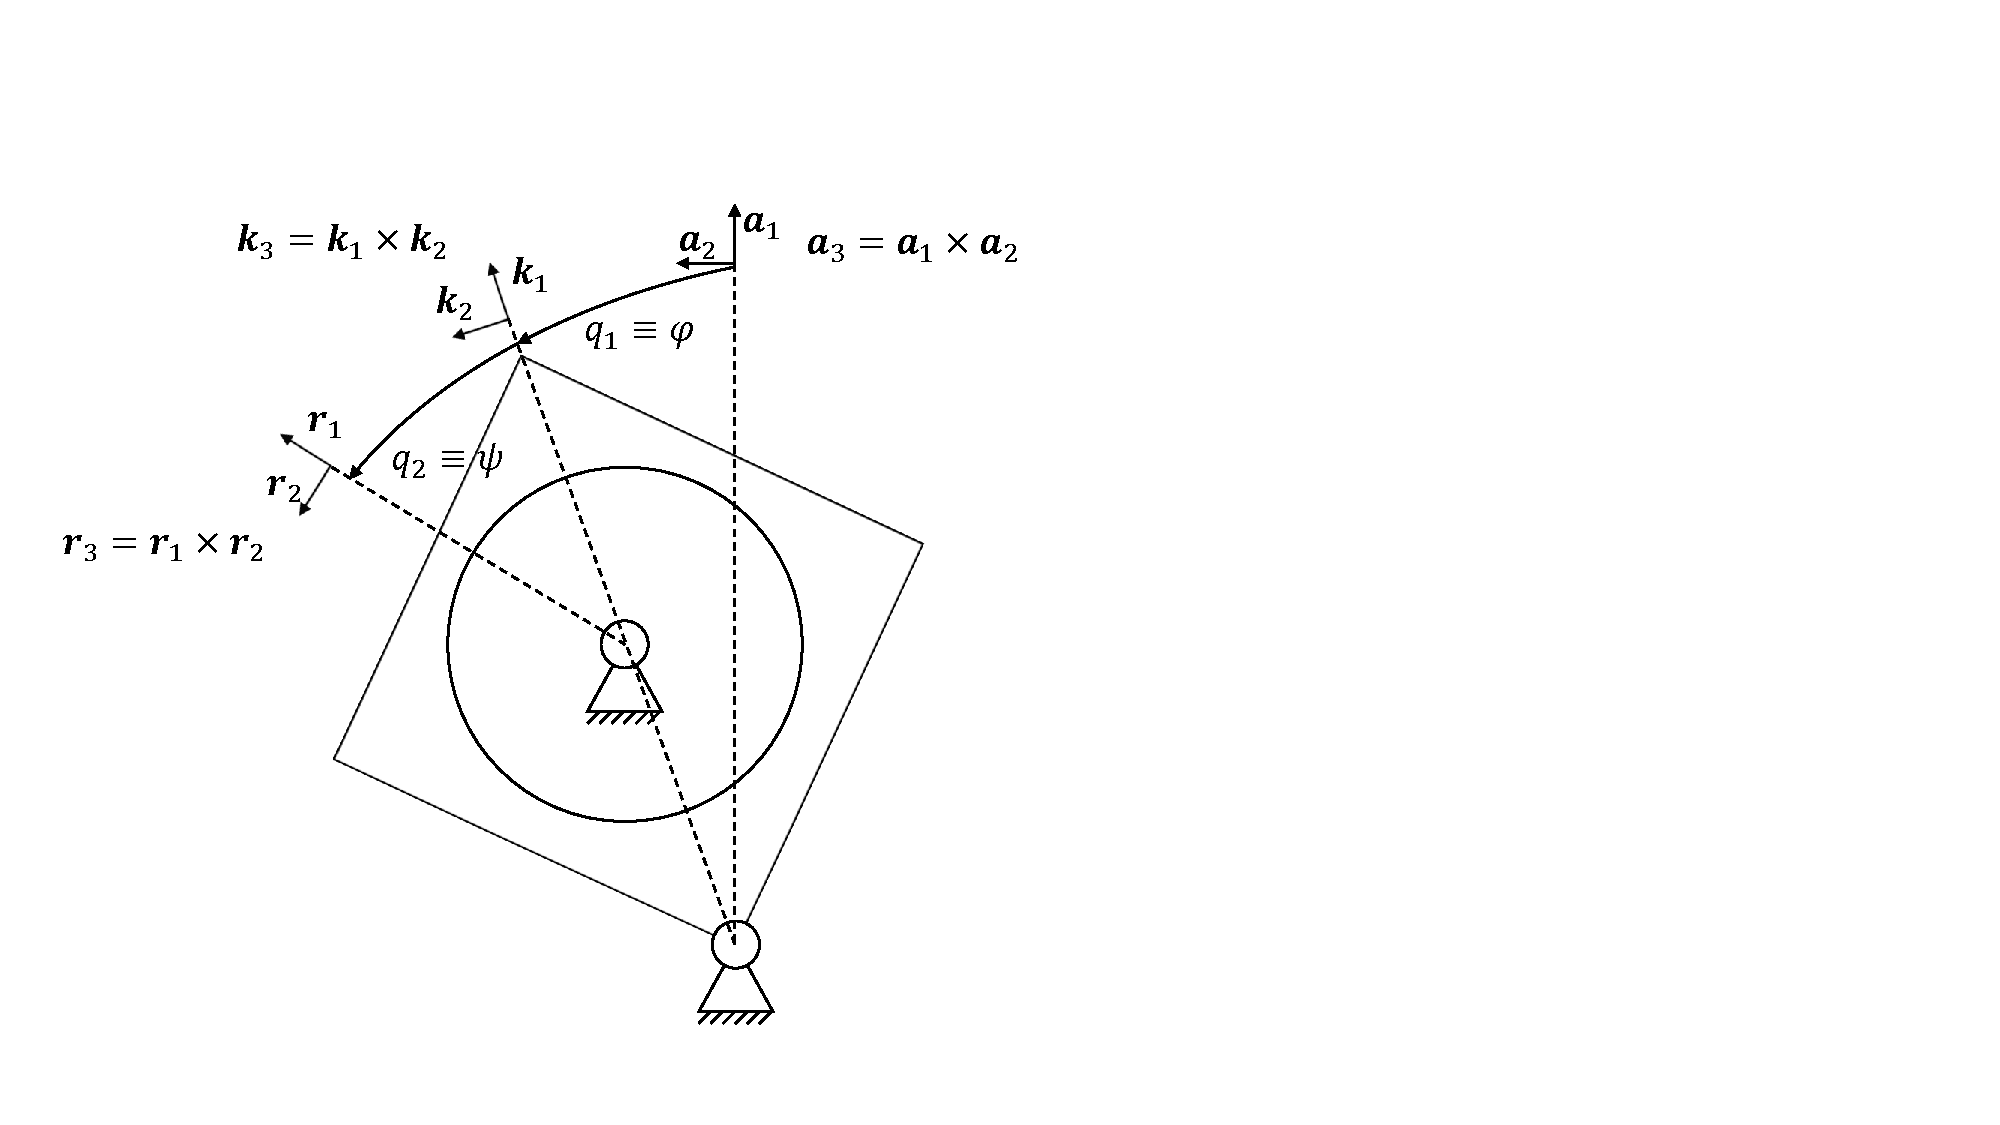
\includegraphics[width=0.6\linewidth, trim={1cm 1.5cm 18cm 3.5cm}, clip]{img/ModellWuerfelseite}
\caption{Kinematikplan des Würfels auf einer Kante, Quelle: eigene Darstellung}
\label{skizze_dynamik_edge}
\end{figure}

Um die Körper des Systems zu modellieren werden im nächsten Schritt die Bezugssysteme $A$, $K$ und $R$ eingeführt, wobei ein beliebiges Bezugssystem $B$ durch drei Vektoren $\bs{b_i} \ i \in \{1,2,3\}$ definiert wird. Die Vektoren $\bs{b_i}$ werden als Vektorbasis bezeichnet.\footnote{Allgemein genügen drei linear unabhängige Vektoren als Vektorbasis, allerdings werden in dieser Arbeit ausschließlich paarweise orthogonale Einheitsvektoren verwendet, da diese eine einfachere Handhabung ermöglichen. Deshalb wird im weiteren Verlauf nicht explizit erwähnt, dass es sich bei den Vektorbasen um paarweise orthogonale Einheitsvektoren handelt.} In diesem Fall ist $A$ ein Intertialsystem, das heißt die Ausrichtung der Vektoren $\bs{a_i}$ ist konstant. Deshalb wird $A$ bzw. dessen Vektorbasis auch als raumfest bezeichnet. Bei $K$ handelt es sich um ein körperfestes Bezugssystem, die Vektoren $\bs{k_i}$ sind an dem Würfelgehäuse fixiert und ändern ihre Ausrichtung in Abhängigkeit von $\varphi$. Das Bezugssystem $R$ ist ebenfalls körperfest, wobei die Vektorbasis an der Schwungmasse fixiert ist. Foglich beschreiben die Koordiaten $\varphi$ und $\psi$ die Rotation von $K$ relativ zu $A$ bzw. von $R$ gegenüber $K$. Mittels eines Bezugssystems kann ein bliebiger Vektor als Linearkombination der Vektorbasis dargestellt werden. Als Beispiel sei der Ortsvektor $\bs{c}$ des Würfelschwerpunktes geannt, wobei das verwendete Bezugssystem durch den vorangehenden Superskript gekennzeichnet wird.
\begin{equation}
\bs{c} = l_C \cdot \bs{k}_1 + 0 \cdot \bs{k}_2 + 0 \cdot \bs{k}_3 = \vecBS{K}{l_C}{0}{0}
\end{equation}
Um nun die Komponenten $\alpha_i$ des Vektors $\bs{c}$ in dem Bezugssystem $A$ zu erhalten, muss das Skalarprodukt $\inProd{\bs{a}_i}{\bs{c}}$ berechnet werden. Wird dieser Ansatz auf alle drei Komponenten appliziert ergibt sich der folgende Zusammenhang.\footnote{Um die allgemeine Gültigkeit der linearen Abbildung zu verdeutlichen wird in dieser Gleichung die Definition $\bs{c}=\vecBS{K}{l_C}{0}{0}\equiv\vecBS{K}{\beta_1}{\beta_2}{\beta_3}$ verwendet.}
\begin{equation}
\begin{split}
\bs{c} &= \vecBS{A}{\alpha_1}{\alpha_2}{\alpha_3} = \inProd{\bs{c}}{\bs{a}_1}\cdot \bs{a}_1 + \inProd{\bs{c}}{\bs{a}_2}\cdot\bs{a}_2 + \inProd{\bs{c}}{\bs{a}_3}\cdot\bs{a}_3 
= \vecBS{A}{\inProd{\bs{c}}{\bs{a}_1}}{\inProd{\bs{c}}{\bs{a}_2}}{\inProd{\bs{c}}{\bs{a}_3}}
\\
&= \vecBS{A}
{\beta_1\cdot\inProd{\bs{a}_1}{\bs{k}_1} + \beta_2\cdot\inProd{\bs{a}_1}{\bs{k}_2} + \beta_3\cdot\inProd{\bs{a}_1}{\bs{k}_3}}
{\beta_1\cdot\inProd{\bs{a}_2}{\bs{k}_1} + \beta_2\cdot\inProd{\bs{a}_2}{\bs{k}_2} + \beta_3\cdot\inProd{\bs{a}_2}{\bs{k}_3}}
{\beta_1\cdot\inProd{\bs{a}_3}{\bs{k}_1} + \beta_2\cdot\inProd{\bs{a}_3}{\bs{k}_2} + \beta_3\cdot\inProd{\bs{a}_3}{\bs{k}_3}}
= \presuper{K}{\begin{pmatrix}
\underbrace{
\begin{bmatrix}
\inProd{\bs{a}_1}{\bs{k}_1} & \inProd{\bs{a}_1}{\bs{k}_2} & \inProd{\bs{a}_1}{\bs{k}_3} \\
\inProd{\bs{a}_2}{\bs{k}_1} & \inProd{\bs{a}_2}{\bs{k}_2} & \inProd{\bs{a}_2}{\bs{k}_3} \\
\inProd{\bs{a}_3}{\bs{k}_1} & \inProd{\bs{a}_3}{\bs{k}_2} & \inProd{\bs{a}_3}{\bs{k}_3}
\end{bmatrix}}_{\equiv \pMat{K}{A}} \cdot \underbrace{\begin{bmatrix}
\beta_1 \\ \beta_2 \\ \beta_3
\end{bmatrix}}_{= \presuper{K}{\bs{c}}}
\end{pmatrix}} 
\\
&= \presuper{A}{\begin{pmatrix}
\begin{bmatrix}c_{\varphi} & -s_{\varphi} & 0 \\ s_{\varphi} & c_{\varphi} & 0 \\ 0 & 0 & 1 \end{bmatrix} \cdot \presuper{K}{\bs{c}} \end{pmatrix}}
\end{split}
\end{equation}
Somit handelt es sich bei der Projekt eines Vektors, der in einem Bezugssystem $E$ dargestellt ist, in das Bezugssystem $F$ um eine lineare Abbildung, welche durch die Abbildungsmatrix $\pMat{E}{F}$ definiert ist. Des weiteren zeigt dieses Beispiel die perspektivische Bedeutung eines Bezugssystem. Wird der Vektor $\bs{c}$ in $K$ dargestellt hängt er lediglich von der Länge $l_C$ ab und ist deshalb konstant. Aus der Perspektive von $A$ ist der Vektor eine Funktion von $\varphi$ und somit variabel. Die Begründung hierfür ist, dass das Intertialsystem $A$ die Bewegung des Würfels im Raum wahrnimmt, wodurch der Ortsvektor des Schwerpunktes variable erscheint. Im Gegensatz dazu bewegt sich das körperfeste Bezugssystem $K$ mit dem Würfel und erfasst dessen Bewegung somit nicht. Dieser Umstand kann genutzt werden, indem ein Vektor zunächst in einer finfachen Form dargestellt und anschließend in das gewünschte Bezugssystem projiziert wird. Als Beispiel dient die Berechnung des Gravitationsmoments $\bs{T}^{K/O}$. Der Erdbeschleunigungsvektor $\bs{g}$ ist im Inertialsystem $A$ konstant und wird von dort in das körperfeste System $K$ transformiert.
\begin{equation}
\begin{split}
\bs{T}^{K/O} = \bs{c}\times m\cdot\bs{g} &= \vecBS{K}{l_C}{0}{0}\times \vecBS{A}{-m\cdot g}{0}{0} = \vecBS{K}{l_C}{0}{0}\times\presuper{K}{\begin{pmatrix}
\pMat{A}{K}\cdot \vecBS{A}{-m\cdot g}{0}{0}
\end{pmatrix}}
\\
&= \vecBS{K}{l_C}{0}{0}\times \vecBS{K}{-c_{\varphi}\cdot m\cdot g}{s_{\varphi}\cdot m\cdot g}{0} = \vecBS{K}{0}{0}{s_{\varphi}\cdot m\cdot g\cdot l_C}
\end{split}
\end{equation}
Dieses Beispiel zeigt, dass die Einführung von Bezugssystemen eine eindeutige Notation und Vorgehensweise zur Berechnung von vektorwertigen Funktionen mit sich bringt. Man möge bei diesem Anwendungsfall zwar argumentieren, dass die trigonometrischen Zusammenhänge des Gravitationsmomentes auch aus der Abbildung \cite{skizze_dynamik_edge} ablesen lassen. Allerdings ist die hier betrachtete Vorgehensweise allgemeingültig und kann auf beliebig komplexe Systeme angewendet werden. Beispielsweise kann das Gravitationsmoment in dem Fall, dass der Würfel auf einer Ecke steht, kaum mehr aus einer Skizze bestimmt werden.

Zur vollständigen Beschreibung der Kinematik müssen die Geschwindigkeiten des Systems ermittelt werden. Als Beispiel für die Ableitung eines Vketors dient wieder der Ortsvektor $\bs{c}$ des Schwerpunktes. Dieser ist aus der Perspektive des Bezugssystem $K$ konstant, folglich verschwindet auch dessen Ableitung bzw. Geschwindigkeit. Wird der Vektor aber in $A$ abgebildet hängt dieser von der Zeitfunktion $\varphi(t)$ ab. Deshalb muss bei der Ableitung eines Vektors das Bezugssystem angegeben werden, aus dessen Perspektive differenziert wird ([Kane], S.25ff). Wenn $\bs{c}$ in $A$ differenziert werden soll, so muss dieser zunächst in $A$ dargestellt und anschließend komponentenweise nach der Zeit abgeleitet werden.
\begin{equation}
\frac{\presuper{A}{d}\bs{c}}{dt} = \frac{d(c_{\varphi}\cdot l_C}{dt}\cdot \bs{a}_1 + \frac{d(0)}{dt}\cdot \bs{a}_3 = \vecBS{A}{-s_{\varphi}\cdot \dot{\varphi}\cdot l_C}{c_{\varphi}\cdot \dot{\varphi}\cdot l_C}{0}
\end{equation}
Analog handelt es sich bei der Geschwindigkeit $\vel{B}{v}{P}$ bzw. Beschleunigung $\vel{B}{a}{P}$ eines Punktes oder Körpers $P$ um eine Bewegung relativ zu einem Bezugssystem $B$. Diese werden wie folgt definiert ([Kane], S.28).
\begin{equation}
\vel{B}{v}{P} = \frac{\presuper{B}{d\bs{p}}}{dt} \hspace{35pt} \vel{B}{a}{P}
\end{equation}
Die selbe Notation wird für Winkelgeschwindigkeiten und -beschleunigungen eingeführt, wobei $\vel{A}{\omega}{B}$ die Winkelgeschwindigkeit bzw. $\vel{A}{\alpha}{B}$ die Winkelbeschleunigung eines Punktes oder Bezugssystems $B$ relativ zu $A$ ist. Die Geschwindigkeit relativ zu einem Inertialsystem wird auch als absolute Geschwindigkeit bezeichnet. Für die Bezugssysteme $K$ und $R$ lassen sich mit Hilfe der Abbildung \cite{skizze_dynamik_edge} die folgenden Winkelgeschwindigkeiten bestimmen, wobei die absolute Winkelgeschwindigkeit eines Bezugssystems die Summe seiner relativen Winkelgeschwindigkeiten ist ([Kane], S.24f).
\begin{equation}
\vel{A}{\omega}{K} = \vecBS{K}{0}{0}{\dot{\varphi}} \hspace{15pt} \vel{K}{\omega}{R} = \vecBS{R}{0}{0}{\dot{\psi}} \hspace{15pt} \vel{A}{\omega}{R} = \vel{A}{\omega}{K} + \vel{K}{\omega}{R} = \vecBS{A}{0}{0}{\dot{\varphi} + \dot{\psi}}
\end{equation}
Der letzte Schritt bei der Untersuchung der Kinematik besteht darin die  generalisierten Geschwindigkeiten zu definieren und daraus die partiellen Geschwindigkeiten zu berechnen. Bei den generalisierten Geschwindigkeiten $u_i$ handelt es sich um skalare Größen deren Anzahl gleich der Zahl der generalisierten Koordinaten ist. Die generalsierten Geschwindigkeiten sind für gewöhnlich abhängig von den Zeitableitungen der generalisierten Geschwindigkeiten $\dot{q}_i$, wobei sie so gewählt werden müssen, dass die Definitionen eindeutig nach den Ableitungen $\dot{q}_i$ aufgelöst werden können. Die Einführung der generalisierten Geschwindigkeiten verfolgt das Ziel, möglichst einfache Ausdrücke für die absoluten Geschwindigkeiten $\vel{A}{\omega}{K}$ und $\vel{A}{\omega}{R}$ und, wie sich im späteren Verlauf zeigen wird, einfachere Ausdrücke der Bewegungsgleichungen zu erhalten. Deshalb werden hier die folgenden Definitionen gewählt.
\begin{equation}
\begin{split}
u_1 \equiv \dot{\varphi} &\hspace{35pt} u_2 \equiv \dot{\varphi} + \dot{\psi} \\
\vel{A}{\omega}{K} = \vecBS{K}{0}{0}{u_1} & \hspace{35pt} \vel{A}{\omega}{R}=\vecBS{K}{0}{0}{u_2}
\end{split}
\end{equation}
Diese Geschwindigkeitsausdrücke können auch in die Form
\begin{equation}
\begin{split}
\vel{A}{\omega}{K} = u_1 \cdot \vel{A}{\omega}{K}_1 + u_2 \cdot \vel{A}{\omega}{K}_2 &\hspace{15pt} \vel{A}{\omega}{R} = u_1 \cdot \vel{A}{\omega}{R}_1 + u_2 \cdot \vel{A}{\omega}{R}_2
\\
\vel{A}{\omega}{K}_1 = \bs{k}_3 \hspace{15pt} \vel{A}{\omega}{K}_2 = 0 &\hspace{15pt}\vel{A}{\omega}{R}_1 = 0 \hspace{15pt} \vel{A}{\omega}{R}_2 = \bs{k}_3
\end{split}
\end{equation}
gebracht werden, wobei die Größen $\vel{A}{\omega}{K}_i$ und $\vel{A}{\omega}{R}_i$ partielle Geschwindigkeiten genannt werden. Diese Zerlegung kann so interpretiert werden, dass die generalisierten Geschwindigkeiten $u_i$ als skalare Größen den Betrag der Bewegung und die entsprechende partielle Geschwindigkeit, als vektorielle Größe, deren Richtung wiedergibt. Die Vorteile diese Zerlegung in generalisierte und partielle Geschwindigkeiten wird sich im folgenden Abschnitt zeigen.
